\documentclass{article}
% PACKAGES %
\usepackage[english]{} % Sets the language
\usepackage[margin=2cm]{geometry} % Sets the margin size
\usepackage{fancyhdr} % Allows creation of headers
\usepackage{xcolor} % Allows the use of color in text
\usepackage{float} % Allows figures and tables to be floats
\usepackage{appendix}
\usepackage{amsmath} % Enhanced math package prepared by the American Mathematical Society
	\DeclareMathOperator{\sech}{sech} % Include sech
\usepackage{amssymb} % AMS symbols package
\usepackage{mathrsfs}% More math symbols
\usepackage{bm} % Allows you to use \bm{} to make any symbol bold
\usepackage{bbold} % Allows more bold characters
\usepackage{verbatim} % Allows you to include code snippets
\usepackage{setspace} % Allows you to change the spacing between lines at different points in the document
\usepackage{parskip} % Allows you alter the spacing between paragraphs
\usepackage{multicol} % Allows text division into multiple columns
\usepackage{units} % Allows fractions to be expressed diagonally instead of vertically
\usepackage{booktabs,multirow,multirow} % Gives extra table functionality
\usepackage[final]{pdfpages} % Allows pdfs to be imported
\usepackage{hyperref} % Allows hyperlinks in the document
\usepackage{rotating} % Allows tables to be rotated
\usepackage{graphicx} % Enhanced package for including graphics/figures
	% Set path to figure image files
	\graphicspath{ {} }
\usepackage{listings} % for including text files
	\lstset{basicstyle=\ttfamily\scriptsize,
        		  keywordstyle=\color{blue}\ttfamily,
        	  	  stringstyle=\color{red}\ttfamily,
          	  commentstyle=\color{gray}\ttfamily,
          	 }		
\newcommand{\tab}{\-\hspace{1cm}}

% Create a header w/ Name & Date
\pagestyle{fancy}
\rhead{\textbf{Mitch Negus} \; 9/22/2017}

\begin{document}
\thispagestyle{empty}

{\bf {\large {NE250 Homework {1} \hfill Mitch Negus\\
		\hspace*{\fill} 9/22/2017\\ }}}
		
%%%%%%%%%%%%%%%%%%%%%%%%%%%%%%%%%% PROBLEM 1 %%%%%%%%%%%%%%%%%%%%%%%%%%%%%%%%%%

\section*{Problem 1}

The number of molecules, $N$, found in a sample of a compound with mass $M$ is 
$$ N(\cdot) = \frac{M(\cdot) N_A}{m(\cdot)} $$
where $m$ is the molar mass of the compound, and $N_A$ is Avogadro's number ($N_A = 6.022 \times 10^{23}$ molecules per mole). Where each actinide isotope is found only once in a molecule of its respective oxide, $N$ also gives the number of atoms of an isotope in the sample. 

To find $N$, we begin by finding the masses of the compounds in the fuel. We can decompose the total mass of the fuel, $M_f$, into its mixed oxide components:
$$ M_f = M(\text{UO}_2) + M(\text{PuO}_2). $$
Given a weight percent for plutonium, $w_{\text{P}}$, we note that $w_{\text{U}} = 1-w_{\text{P}}$ and so calculate the total masses of both the UO$_2$ and the PuO$_2$ to be
$$ M(\text{UO}_2) = (1-w_{\text{P}})M_f	$$
$$ M(\text{PuO}_2) = w_{\text{P}}M_f. $$

We are told that the uranium is all $^{238}$U, so 
$$ M(^{238}\text{UO}_2) = M(\text{UO}_2) = (1-w_{\text{P}})M_f. $$

<<<<<<< HEAD
The weight percents of the plutonium isotope oxides are also given (as a fraction of total plutonium oxide). Using $^{239}\text{PuO}_2$ as an example
$$ M(^{239}\text{PuO}_2) = w_{\text{P}9}M(\text{PuO}_2) = w_{\text{P}9}w_{\text{P}}M_f. $$


Next, we must determine the molar masses of the various oxides. For uranium,
$$ m(^{238}\text{UO}_2) = m(^{238}\text{U}) + 2m(\text{O}), $$
and similarly for plutonium.

When we combine the total and molar masses to determine the total number of atoms for each isotope, we find:\\
\tab 6.69$\times 10^{20} \text{ atoms of }^{238}$U	\\
\tab 4.65$\times 10^{20} \text{ atoms of }^{239}$Pu	\\
\tab 1.45$\times 10^{20} \text{ atoms of }^{240}$Pu	\\
\tab 3.84$\times 10^{19} \text{ atoms of }^{241}$Pu	\\
\tab 1.78$\times 10^{19} \text{ atoms of }^{242}$Pu	\\

(for full calculation, see Jupyter notebook, attached)

%%%%%%%%%%%%%%%%%%%%%%%%%%%%%%%%%% PROBLEM 2 %%%%%%%%%%%%%%%%%%%%%%%%%%%%%%%%%%

\section*{Problem 2}

We use the


\subsection*{\textit{a.})}


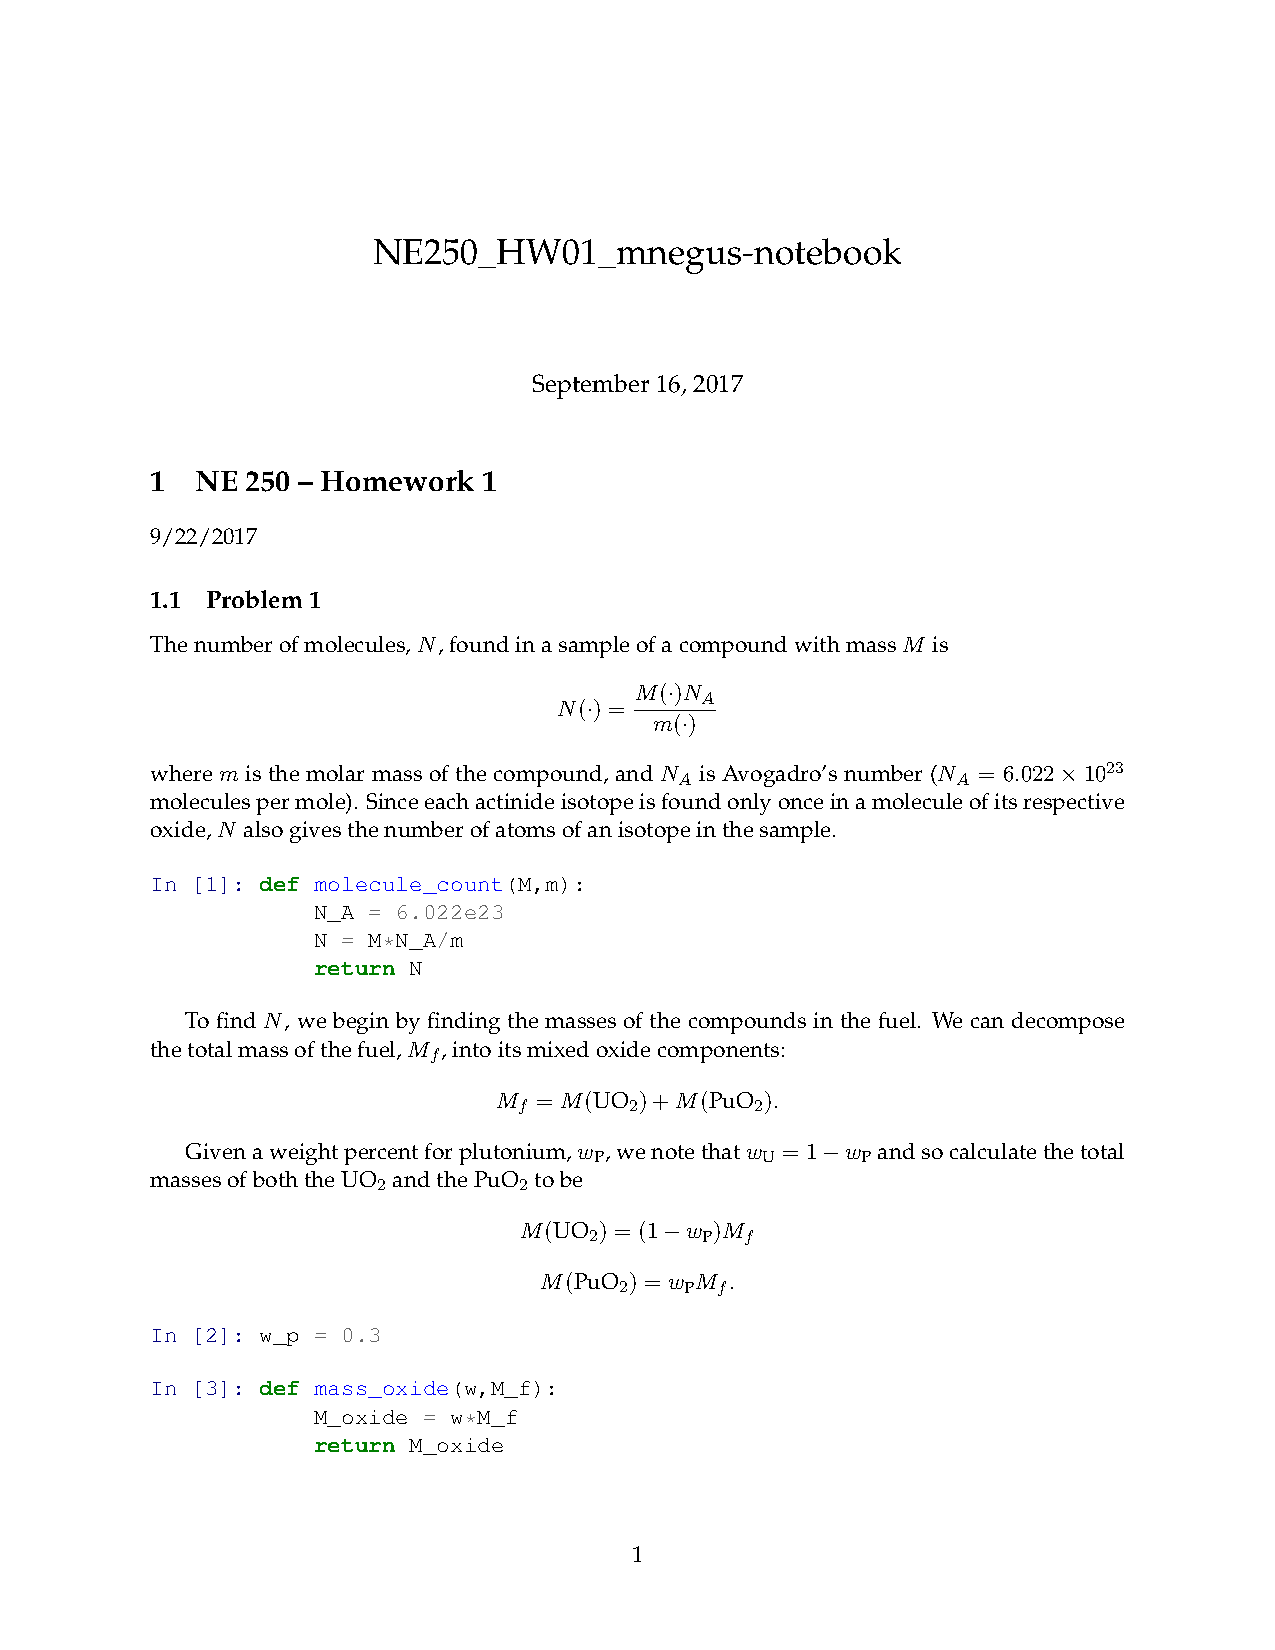
\includepdf[pages=-]{NE250_HW01_mnegus-notebook.pdf}



\end{document}







